\documentclass[a4paper]{report}

%% Language and font encodings
\usepackage[english]{babel}
\usepackage[utf8x]{inputenc}
\usepackage[T1]{fontenc}
\usepackage{graphicx}
\usepackage[english]{babel}
\usepackage[utf8x]{inputenc}
\usepackage[T1]{fontenc}
\usepackage{sectsty}
\usepackage{pdfpages}
\usepackage[section]{placeins}
\usepackage{float}% If comment this, figure moves to Page 2
\usepackage{listings}
\usepackage{caption}
\usepackage{subcaption}

%% Sets page size and margins
\usepackage[a4paper,top=3cm,bottom=2cm,left=3cm,right=3cm,marginparwidth=1.75cm]{geometry}

%% Useful packages
\usepackage{amsmath}
\usepackage{graphicx}
\usepackage[colorinlistoftodos]{todonotes}
\usepackage[colorlinks=true, allcolors=blue]{hyperref}

\title{Your Paper}
\author{You}

\begin{document}
\maketitle
\tableofcontents






\chapter{Security}
We need to consider atacks on Confidentiality,Integrity and Availability.AIacks need to be monitored andd etected, resisted where possible, otherwise we may need some other form of reaction, eventually we should be able to fully recover.
\section{Important QA's}
\begin{enumerate}
\item \textbf{Confidentiality} - Only those who should have accessare given access
\item \textbf{Integrity} -  Data or services are not subject to unauthorised manipulation.
\item \textbf{Availibility} -  The system is availble for legitimate use.
\item \textbf{Security Mechanisms} Authentication, Authorisation, non-repudation
\end{enumerate}

\section{Security Scenario Components}
\subsection{Generic Example}
\begin{figure}[h]
\centering 
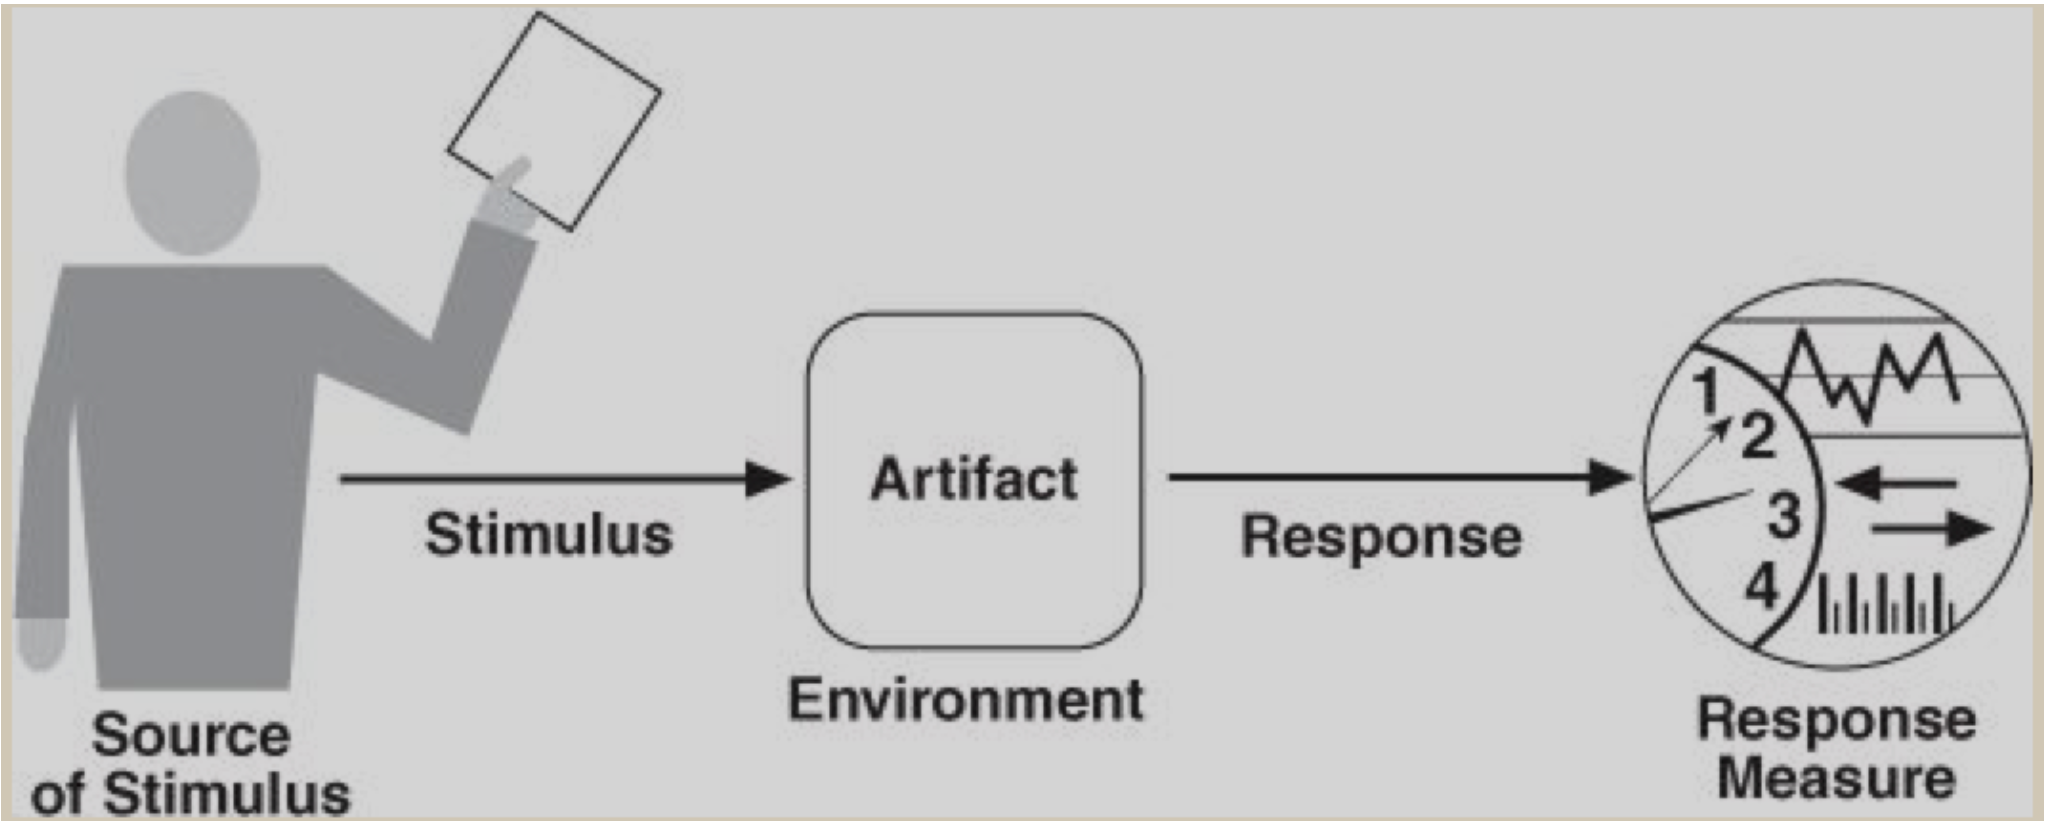
\includegraphics[scale=0.3]{aimages/genreralqascenario.png}
\caption{\label{tab:widgets} QA Scenario Components}
\end{figure}

\begin{itemize}
\item \textbf{Source}- Humans or systems that may or may not have been identified and can be either inside or outside the organisation
\item \textbf{Stimulus}- Unauthorized attempt to access, Manipulate or disable the artifact.
\item \textbf{Artifact}- System services, data, components, data produced or consumed by the system.
\item \textbf{Environment}- online, offline, connected to network, disconnected to network, behind firewall, fully/partially operating, not operational
\item \textbf{Response}- Transaction carried out s.t: Data or services protected from unauthorised access, no data manipulation without authorization, parties in a transaction are identified with assurance, Par'es cannot repudiate their participation, Data, resources etc are available for legititimate use, Appropriate people are notified when threat is identified.
\item \textbf{Response Measure}- assessment of the degree of compromise, temporal and spatial data on the compromise, how many atacks were resisted, how much data is vulnerable
\end{itemize}

\section{More Concrete example}
Assume a more concrete example fo Denial of Service. The components could be:
\begin{itemize}
\item \textbf{Source}- A wide ranfe of systems with different IP.
\item \textbf{Stimulus}- Access to the service provided
\item \textbf{Artifact}- The service we are concerened with
\item \textbf{Environment}- Normal operation
\item \textbf{Response}- Detect Normal Load
\item \textbf{Response Measure}- Mode of operation is changed to ensure normal service to trusted IP addresses.!!what?!!
\end{itemize}

\section{Security Architecture tactics}
Tactics are a high-level way of categorizing possible protection against aIack.
\begin{figure}[h]
\centering 
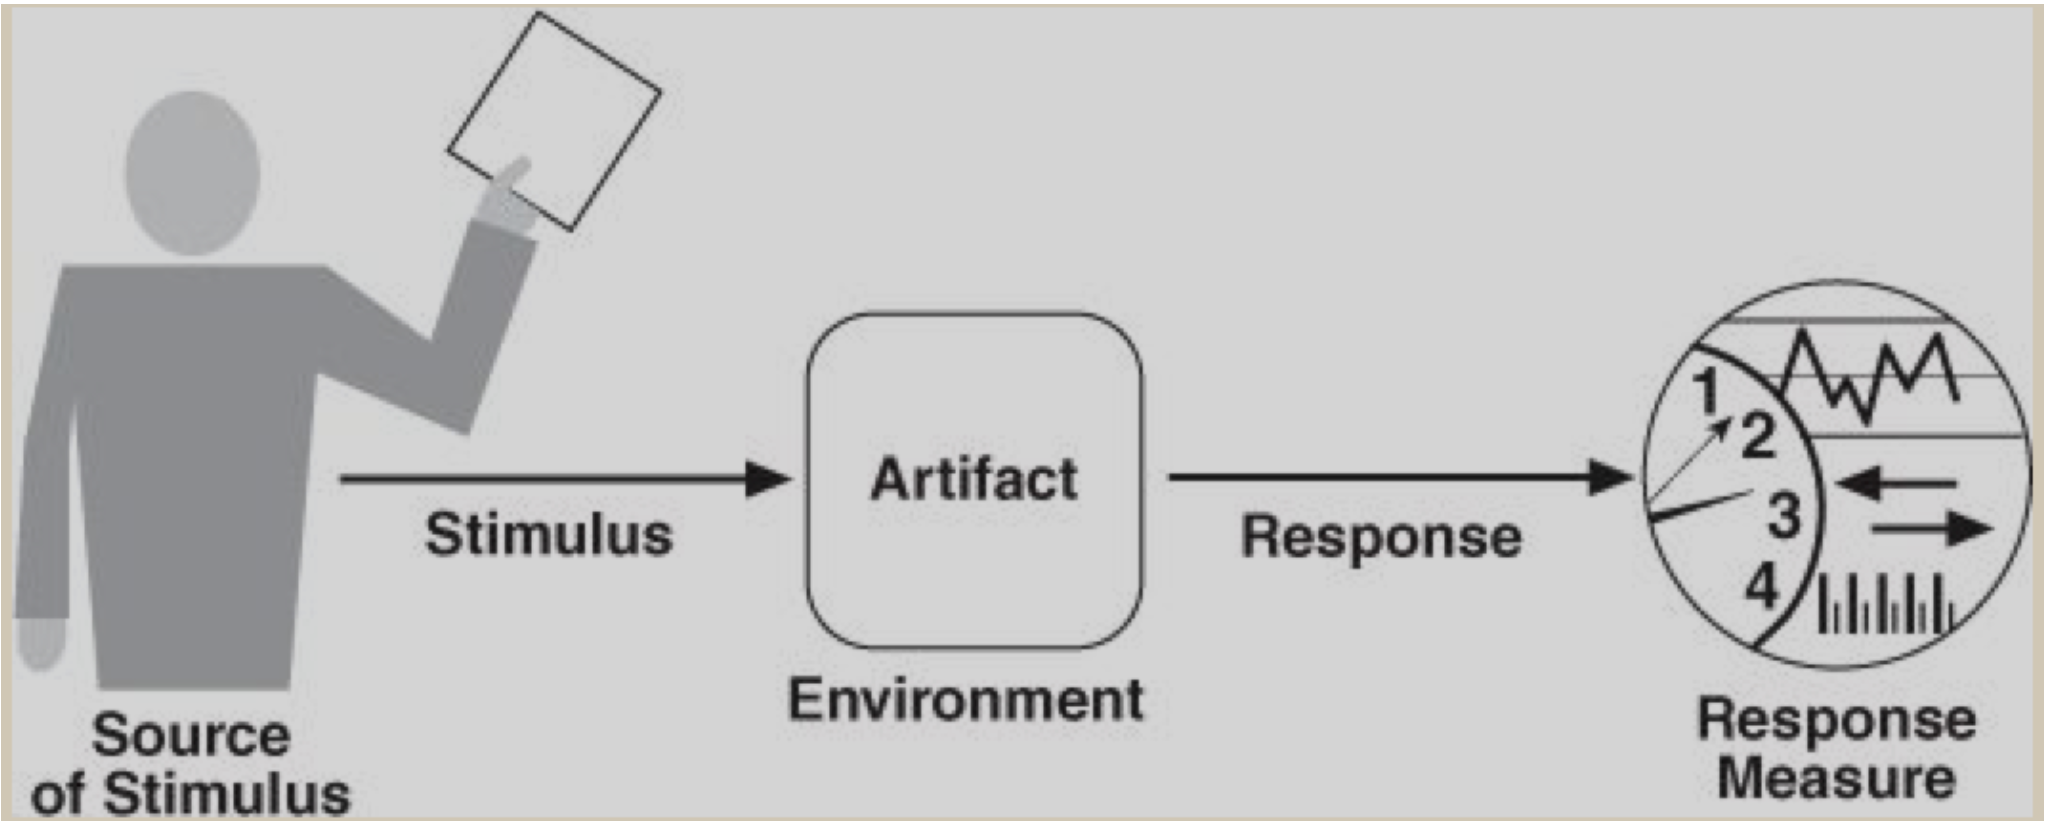
\includegraphics[scale=0.3]{aimages/genreralqascenario.png}
\caption{\label{tab:widgets}Security Architectural Tactics}
\end{figure}

\section{Architectural Design Decisions}
\subsection{Allocation of resposibilities}
For security-system responsibilities do the following:
\begin{itemize}
\item Ensure all actors have identities(like roles)
\item Authenticate identities to apprppriate actors.
\item Check and Ensure Authorization
\item Ensure Data Encryption
\item Log attempts, successes, failures and other senitive oprations.
\end{itemize}
\subsection{Coordination Model}
The following things in the coordination model need to be acoounted for:
\begin{itemize}
\item Ensure coordination mechanisms use authentication and 
\item Ensure the coordination model is not vulnerable to tampering, interception, impoersonation.
\item The model data involved is encrypted.
\item Monitor level of demand for communication to identify excessive demands
\end{itemize}
\subsection{Data Model}
\begin{itemize}
\item Ensure There is a vald data model that disallows invalid data flows.
\item Ensure Logging of access, modification and attempted access or modification.
\item Data is protected in flight at rest using appropriate encryption
\item Ensure appropriate backup/recovery mechanisms are in place. 
\end{itemize}

\subsection{Mapping among Architectural Elements}
\begin{itemize}
\item Explore and be wary be wary how different mappings change the way users can access resources.
\item Ensure for all the mappings, the responsibilities(authorization, logging,encryption etc) are preserved.
\item Ensure recovery from attack is possible.
\end{itemize}
\subsection{Resource Management}
\begin{itemize}
\item explore teh overheads resulting from responsibilities(logging, encryption, recovery etc).
\item Analyse how a user can make demands on a critical resource.
\item Make sure malicious use of resources is detected and managed.
\item Identify and manage the potential fot corruption/contamination.
\item explore the potential for resource use to be used as a covert channel to trnasmit data.
\item limite resources used to manage sttemps at unauthorised use !!surely depends on use case?!!.
\end{itemize}
\subsection{Binding Time}
\begin{itemize}
\item Explore the consequesces of varying binding times on the ability to trust actor or components.
\item place mechanisms to ensure trust given in bindin time.
\item Explore impact on resource use, capacity/throughput, response time.
\item Ensure the time bindings are ensured with all resposibilities(authorization, logging,encryption etc).
\item Explore the potential of variation in binding time as a covert channel.
\end{itemize}

\subsection{Choices of Technologies}
\begin{itemize}
\item  Ensure limitations of technologies are understood and the potential for future compromise is well identified.
\item Ensure your chosen technologies support the tactics you want to deploy to protect the system.
\end{itemize}
\end{document}
